\documentclass[]{article}
\usepackage{amsmath}
\usepackage{amsfonts}
\usepackage{amssymb}
\usepackage{hyperref}
\usepackage{gensymb}
\usepackage{graphicx}
\usepackage{svg}
\usepackage{bbding}
\usepackage{mathtools}
\usepackage{centernot} % not parallel, etc.
\usepackage{lmodern}
\usepackage{morewrites}
\usepackage{xcolor,sectsty} % colorful sections
\usepackage[left=10mm, top=10mm, right=10mm, bottom=20mm, nohead]{geometry}
%\usepackage{bigints}
\usepackage{dsfont} %mathbb 1
\usepackage{esint} % beatiful integrals
\usepackage{physics}


\DeclareFontFamily{OMX}{lmex}{}
\DeclareFontShape{OMX}{lmex}{m}{n}{<-> lmex10}{}


%colors of sections
\definecolor{secfont}{RGB}{46,116,181}
\definecolor{subfont}{RGB}{146,23,57}
\definecolor{parfont}{RGB}{19,127,43}
\definecolor{subparfont}{RGB}{7,11,100}

\subsectionfont{\color{subfont}}
\sectionfont{\color{secfont}}
\paragraphfont{\color{parfont}}
\subparagraphfont{\color{subparfont}}

%\usepackage{babel}[english]
%opening
\title{114036 - Statistical and Thermal Physics}
\author{Amit Keren}
% Wednesday 304, 16:00
% send notes
% Midterm - 5 lists, Final 10 lists
% Book Kittel Statermit

\parindent=0em
\begin{document}


\maketitle

\begin{abstract}

\end{abstract}

%\tableofcontents
\section{Introduction}
\paragraph{History}
\begin{itemize}
	\item First, thermodynamics was developed, before atoms were known to exist.
	\item Statistical physics.
	\item Quantum physics. 
\end{itemize}
In the course, the order is the opposite.
\subsection{}
Suppose we have two balls of diameter $d$. If both are on the bottom, total energy is 0. If one i son the other, total energy is $mgd$.

\begin{center}
	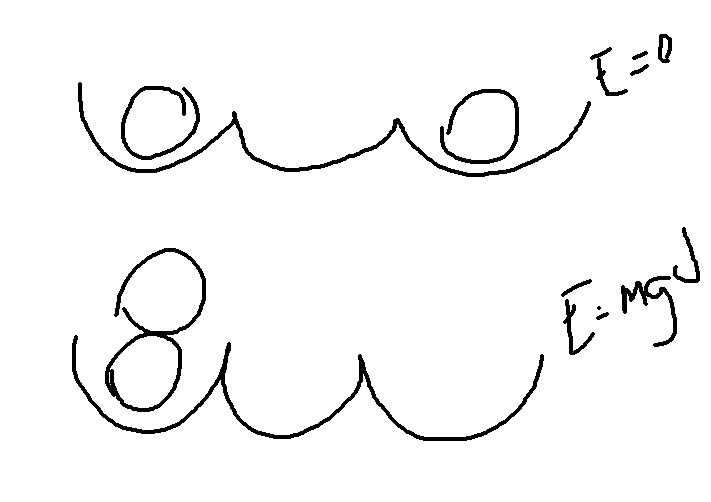
\includegraphics[width=0.5\linewidth]{./lect1/pic1.png}
	
	\begin{tabular}{c|c|c}
		Number of state & Degeneracy & Energy \\\hline
		0 & 3 & 0 \\
		1 & 3 & $mgd$ \\
		2 & 0 & $2mgd$ \\
	\end{tabular}
\end{center}
\paragraph{Paramagnetism}
Define magnetic moment as $\vec{m} = I \vec{a}$.
For magnetic filed energy is $U = -\vec{B} \cdot \vec{m} = - \vec{B} \dot \vec{\mu}$.

Suppose we a have a system of a big amount of current loops, each of which can have one of two directions - clockwise or counterclockwise. For example

\begin{center}
	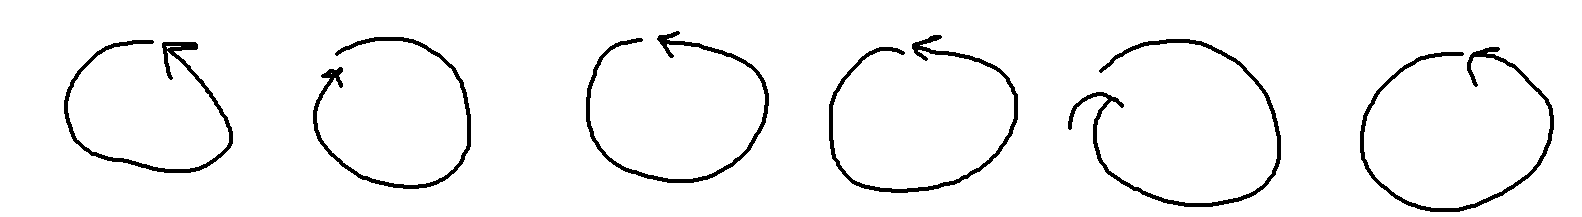
\includegraphics[width=0.5\linewidth]{./lect1/pic2.png}
\end{center}
To calculate total magnetic momentum we just sum all of the moments, which are either $\mu$ or $-\mu$. In upper example, $M = \sum_i \mu_i = 2\mu$.


The total number of possible states is $2^N$. The possible energy is $M = (N-2N_d)\mu$ where $N_d$ is number of down-facing loops of current. Number of different states with sam energy is $$\binom{N}{N_d} = \frac{N!}{N_d!N_u!}$$

Now, for even $N$, define 
$$2S = N_u -N_d$$
Then
$$\binom{N}{N_d} = \frac{N!}{(\left(\frac{1}{2} N - S\right)!(\left(\frac{1}{2} N + S\right)!}$$
and the energy
$$U = -2S\mu B \Rightarrow S = -\frac{U}{2\mu B}$$
The degeneracy of the state thus is
$$g(N,S) = \frac{N!}{\left(\frac{1}{2} N - \frac{U}{2\mu B}\right)!(\left(\frac{1}{2} N + \frac{U}{2\mu B}\right)!}$$ 
\paragraph{Particles on shelves (quantum oscillator)}
Suppose we have equally-distant shelves, and energy distance between two shelves is $\epsilon_0$:
\begin{center}
	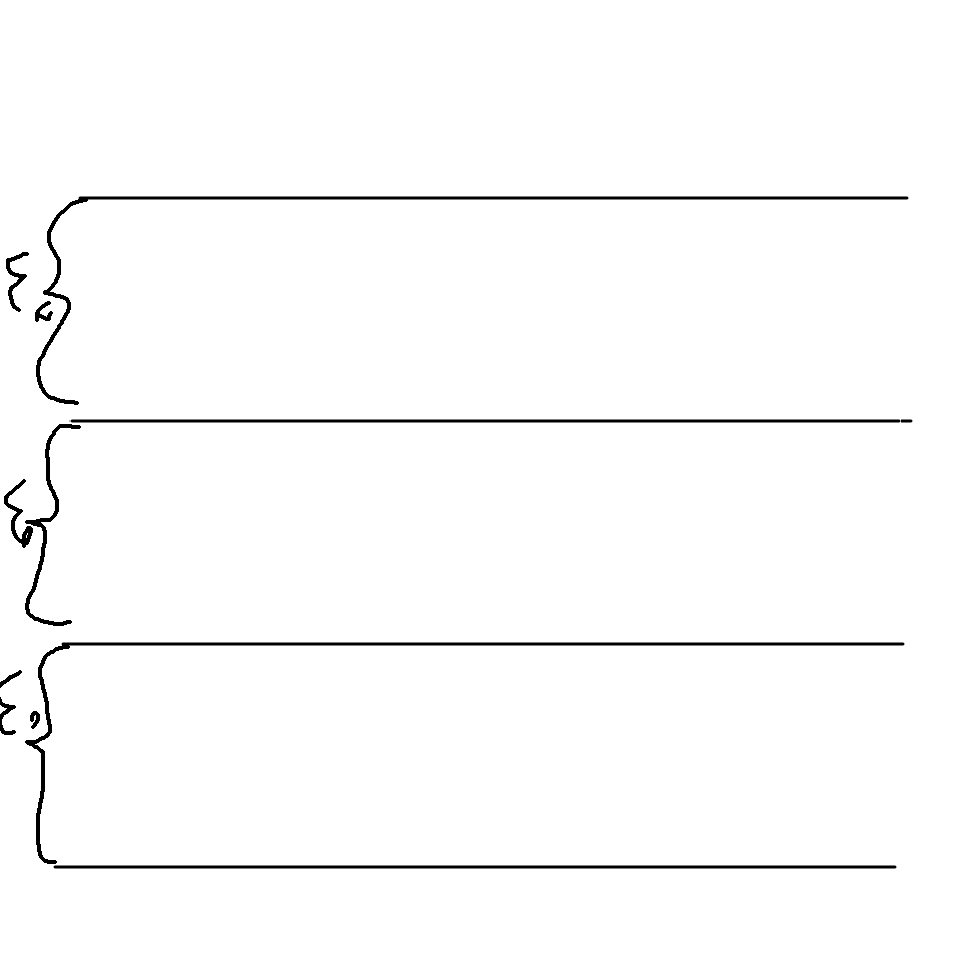
\includegraphics[width=0.5\linewidth]{./lect1/pic3.png}
\end{center}
Define $n=\frac{U}{\epsilon_0}$ which is amount of energy we have (it comes in quantas is degeneracy? What is degeneracy? It is combinations of$N$ out $n$ with returns:
$$g(N,u) = \frac{(n+N-1)!}{n!(N-1)!} = \frac{\left(N+\frac{U}{\epsilon_0} - 1\right)!}{\left(\frac{U}{\epsilon_0}\right)!(N-1)!}$$

\paragraph{Particles on shelves with quadratic distances (particles in box)}
Now suppose distances goes as square of number opf shelve ($\epsilon_0$, $4\epsilon_0$, ...). This problem doesn't have analytical solution. But we can find solution manually. For example, to find $g(6,18\epsilon_0)$. The only option is 2 boxes on first energy level $U=\epsilon_0$ and 4 on second energy level, thus 
$$g(6, 18\epsilon_0) = \binom{6}{2}=15$$  
\paragraph{1D box with particles}
Now we want to calculate kinetic energy:
$$E = \frac{p^2}{2m}$$
Since we can't do much with continuous values (there is infinite number of options), lets divide both momentum and position into discrete intervals of size $w$ and $l$ correspondingly. Now, the position is independent on energy, but there are only two options for momentum - $\pm \sqrt{2mE}$. Thus degeneracy is
$$g(1, E) = 2\frac{L}{l} $$
\paragraph{2D box}
We now divide position in momentum into intervals of length $l$ and $w$ in both directions. Position is still arbitrary, and momentum lies on a circle of radius $2mE$. However, its hard to calculate.

Lets define instead $S(1,E)$ - number of states with energy \textit{less} than $U$. For 1-dimensional case 
$$S(1,E)  = \frac{L}{l} \cdot 2 \cdot \frac{\sqrt{2mE}}{w} = \frac{1}{lw} \int_{-\frac{L}{2}}^{\frac{L}{2}} ds \int_{-\sqrt{2mE}}^{\sqrt{2mE}} ds$$
In 2D we get, for box of area $A$
$$S(1,E) = \frac{A}{l^2} \cdot \frac{2\pi m E}{w^2} =  \frac{1}{l^2w^2} \int_{-\frac{L}{2}}^{\frac{L}{2}}dx\int_{-\frac{L}{2}}^{\frac{L}{2}}dy \iint\limits_{|p| < \sqrt{2mE}} d^2p$$
$$S(1,E) = \frac{V}{l^3} \cdot\frac{4\pi (2 m E)^{\frac{3}{2}}}{3w^3}$$
We denote $h=lw$.
Now note that $G(n, U) = \pdv{S(n,U)}{U}$.

\paragraph{Two distinguishable particles in 1D}

While positions are independent, there is dependence between $p_1$ and $p_2$:
$$\frac{p_1^2}{2m}+\frac{p_2^2}{2m} + E$$
We can note that
$$S_{2D}(1,U) = S_{1D} (2, U)$$

\paragraph{$N$ particles in $D$ dimensions}
$$S_D(N,U) = \frac{1}{h^{DN}} \int\limits_{\va{x}_1 \in V} \dd[D]{x_1} \: \dots  \int\limits_{\va{x}_n \in V} \dd[D]{x_n}  \idotsint\limits_{\sum_{i=1}^n \va{p}_i^2 \leq 2mU} \dd[D]{p_1} \dots \dd[D]{p_n}$$

\subparagraph{Ball volume in dimension $d$}
Define gamma function. For $\alpha > 0$
$$\frac{1}{\alpha} = \int_0^\infty \dd{x} e^{-x\alpha}$$
Differentiating $n$ times by $\alpha$ (and dividing by $(-1)^n$:
$$\frac{N!}{\alpha^{N+1}} = \int_0^\infty \dd{x} x^N e^{-x\alpha}$$
By substituting $\alpha = 1$:
$$N! = \int_0^\infty \dd{x} x^N e^{-x}$$
Thus define 
$$\Gamma(N+1) = \int_0^\infty \dd{x} x^n e^{-x}$$

Define area of $d$-dimensional sphere of radius $R$ as
$$A_d = S_d \cdot R^{d-1}$$
Define also
$$I_d = \left(\int_{-\infty}^{\infty} \dd{x} e^{-x^2}\right)^d$$
On one hand $I_D = \pi^{\frac{d}{2}}$, on the other hand
$$I_d = \int_{-\infty}^{\infty} \dd{x_1}  e^{-x^2} \int_{-\infty}^{\infty} \dd{x_2}  e^{-x^2} \dots \int_{-\infty}^{\infty} \dd{x_n}  e^{-x^2} = \int_{-\infty}^{\infty} \dd{x_1}\dd{x_2}\dots \dd{x_n}   e^{-\sum_{i=1}^n x_i^2}$$
For $R=\sum_{i=1}^n x_i^2$:
$$I_D = \int_0^\infty \dd{R} S_d R^{d-1} e^{-R^2}$$
(Note that when we perform integral over angular dimensions we acquire exactly $S_d$ from Jacobean).

For $y=R^2$, $\dd{y}=2R\dd{R}$:
$$\int_0^\infty \frac{dy}{2\sqrt{y}} S_d y^{\frac{d-1}{2}} e^{-y} = \frac{S_d}{2} \int_{0}^{\infty} y^{\frac{d}{2} -1} e^{-y} dy = \frac{S_d}{2} \Gamma\left(\frac{d}{2}\right)$$
Thus
$$\frac{S_d}{2} \Gamma\left(\frac{d}{2}\right) = \pi^{\frac{d}{2}} $$
i.e.\
$$S_d = \frac{2\pi^{\frac{d}{2}}}{\Gamma\left(\frac{d}{2}\right)}$$

Now the volume of $d$-dimensional ball
$$V_d = \int_0^R \dd{r} \frac{2\pi^{\frac{d}{2}}}{\Gamma\left(\frac{d}{2}\right)} r^{d-1}= \frac{\pi^{\frac{d}{2}}}{\Gamma\left(\frac{d}{2}\right)} \frac{r^{d}}{\frac{d}{2}}= \frac{\pi^{\frac{d}{2}}r^{d}}{\Gamma\left(\frac{d}{2}+1\right)}$$

Back to our particles:

$$S_D(N,U) = \frac{1}{h^{DN}} \int\limits_{\va{x}_1 \in V} \dd[D]{x_1} \: \dots  \int\limits_{\va{x}_n \in V} \dd[D]{x_n}  \idotsint\limits_{\sum_{i=1}^n \va{p}_i^2 \leq 2mU} \dd[D]{p_1} \dots \dd[D]{p_n} = \frac{L^{DN} \pi^{\frac{DN}{2}} (2mU)^{\frac{DN}{2}}}{h^{DN} \Gamma\left(\frac{DN}{2}+1\right)} = \left(\frac{L}{h}\right)^{DN}\frac{  (2\pi mw)^{\frac{DN}{2}}}{\Gamma\left(\frac{DN}{2}+1\right)}$$

Thus in our world 
$$S_3(N,U) = \frac{V^{N} \pi^{\frac{3N}{2}} (2mU)^{\frac{3N}{2}}}{h^{3N} \Gamma\left(\frac{3N}{2}+1\right)}$$
And
$$G_3(N,U) = \pdv{S_3(N,U)}{U} = \frac{V^{N} \pi^{\frac{3N}{2}} (2mU)^{\frac{3N}{2}-1} \cdot \frac{3}{2}N \cdot 2m}{h^{3N} \Gamma\left(\frac{3N}{2}+1\right)} = \frac{3V^{N} \pi^{\frac{3N}{2}} (2mU)^{\frac{3N}{2}-1}mN}{h^{3N} \Gamma\left(\frac{3N}{2}+1\right)}$$

\paragraph{Integral approximation with steepest descent}
Suppose we want calculate 
$$I = \int \dd{x} e^{N \phi(x)}$$
for some big $N$ and $x_{max}$ is maximum of $\phi$:
$$I \approxeq \int \dd{x} \exp\left[N \left(\phi(x_{max}) - \frac{1}{2} \left| \phi''(x_{max}) \right| (x-x_{max})^2 + \frac{1}{3!} \phi'''(x_{max} ) (x-x_{max})^3 \right)\right]$$
Then, substituting $y=\sqrt{N}(x-x_{max})$
$$I = e^{N\phi(x_{max})} \int \frac{\dd{y}}{\sqrt{N}} e^{-\frac{1}{2} |\phi''(x_{max})| y^2 + \frac{1}{3!}\phi''' \left(x_{max}\right)\frac{y^3}{\sqrt{N}}}$$
Since $N$ is big, $\frac{1}{3!}\phi''' \left(x_{max}\right)\frac{y^3}{\sqrt{N}}$ is negligible (and higher orders too):
$$I =  e^{N\phi(x_{max})} \sqrt{\frac{2\pi}{N |\phi''(x_{max})|}}$$

\subparagraph{Example}
Lets approximate $n!$:
$$\Gamma(n+1) = \int_0^\infty \dd{x} x^N e^{-x} = \int_0^\infty \dd{x} e^{N \left( \ln x - \frac{x}{N}\right)}$$
Thus $\phi(x) = \ln x - \frac{x}{N}$, and
$$\phi'(x)  = \frac{1}{x} - \frac{1}{N}$$
i.e., $x_{max} = N$. And
$$\left|\phi''(x) \right| = \frac{1}{x^2} $$
$$\Gamma(n+1) = \int_0^\infty \dd{x} x^N e^{-x} = \int_0^\infty \dd{x} e^{N \left( \ln x - \frac{x}{N}\right)} \approxeq e^{N\left( \ln N - 1\right)} \sqrt{\frac{2\pi}{N \frac{1}{N^2}}} = N^N e^{-N} \sqrt{2 \pi N}$$
which is Stirling approximation. We usually want to take logarithm:
$$\ln (N!) \approxeq N\ln N - N + \frac{1}{2} \ln (2\pi N)$$
\paragraph{Example}
Back to example with up and down particles:
$$g(N,S) = \frac{N!}{N_{\uparrow}!N_\downarrow!}$$
where $2S = N_\uparrow - N_\downarrow$ and $N= N_\uparrow + N_\downarrow$
$$\ln g = \ln N! - \ln N_\uparrow ! - \ln N_\downarrow!$$
$$\ln N! = \frac{1}{2} \ln 2\pi + (N+1) \ln N - \frac{1}{2} \ln N - N$$
Substituting
$$\ln N! = \frac{1}{2}ln \frac{2\pi}{N} + \qty(N_\uparrow + \frac{1}{2} + N_\downarrow + \frac{1}{2}) \ln N - (N_\uparrow + N_\downarrow)$$
in addition
$$\ln N_\uparrow! = \frac{1}{2} \ln 2\pi + \qty(N_\uparrow + \frac{1}{2}) \ln N_\uparrow - N_\uparrow$$
$$\ln N_\downarrow! = \frac{1}{2} \ln 2\pi + \qty(N_\downarrow + \frac{1}{2}) \ln N_\downarrow - N_\downarrow$$
so
$$\ln g = \frac{1}{2}ln \frac{1}{2\pi N}  - \qty(N_\uparrow - \frac{1}{2}) \ln \frac{N_\uparrow}{N}   - \qty(N_\downarrow + \frac{1}{2}) \ln \frac{N_\downarrow}{N} $$
Now since
$$\ln \frac{N_\uparrow}{N} = \ln(\frac{1}{2} + \frac{2S}{2N}) = \ln\frac{1}{2}\qty(1 + \frac{2S}{N}) = \ln \frac{1}{2} + \ln(1+\frac{2S}{N})$$
If $S \ll N$
$$\ln \frac{N_\uparrow}{N}  = -\ln 2 + \frac{2S}{N} - \frac{2S^2}{N^2}$$
similarly
$$\ln \frac{N_\downarrow}{N}  = -\ln 2 - \frac{2S}{N} + \frac{2S^2}{N^2}$$
Thus
$$\ln g = \frac{1}{2}ln \frac{1}{2\pi N}  - \qty(\frac{1}{2}N + S - \frac{1}{2}) \qty(-\ln 2 + \frac{2S}{N} - \frac{2S^2}{N^2})  - \qty(\frac{1}{2}N - S + \frac{1}{2}) \qty(-\ln 2 - \frac{2S}{N} +  \frac{2S^2}{N^2}) $$
i.e.,
$$\ln g = \frac{1}{2}ln \frac{2}{\pi N}  + N \ln 2 -\frac{2S}{N} + \order{\frac{S^3}{N^2}}$$
$$g(N,S) = \qty(\frac{2}{\pi N})^{\frac{1}{2}} 2^N e^{-\frac{2S^2}{N}}$$
And if use energy,
$$g(N, U) = \qty(\frac{2}{\pi N})^{\frac{1}{2}} 2^N e^{-\frac{2U^2}{(\mu B)^2N}}$$

Now since number of configurations is $2N$, 
$$\rho(S) = \qty(\frac{2}{\pi N})^{\frac{1}{2}} e^{-\frac{2S^2}{N}} $$
Which is normal distribution with mean $0$ and standard deviation $\frac{\sqrt{N}}{2}$.

Lets check the standard deviation of actual $S$:
$$\langle (2S)^2 \rangle = \left\langle \qty(\sum_i N_i) \right\rangle = \left\langle \sum_{i,j} N_iN_j \right\rangle = \left\langle \sum_i N_i^2 \underbrace{\sum_{i\neq j} N_iN_j}_{0 \: \text{from independence}} \right\rangle  =\left\langle \sum_i N_i^2\right\rangle = N$$
Thus variance of $2S$ is $N$ and variance of $S$ is $\frac{N}{4}$. (This is immediate from CLT).
Now, relative standard deviation
$$\frac{\langle (2S)^2 \rangle}{N} = \frac{1}{\sqrt{N}}$$

For that lets define new variable $X = \frac{2S}{N}$, then
$$\rho(X) = \qty(\frac{N}{2\pi})^{\frac{1}{2}} e^{-\frac{NX^2}{2}}$$
\paragraph{Ergodic hypothesis}
For closed system ($B$, $E$, $N$, $V$ are constant) there is equal probability to acquire any of possible states. Such ctates are called \textbf{microcanonical ensemble}.

Example of exceptions:
\begin{center}
	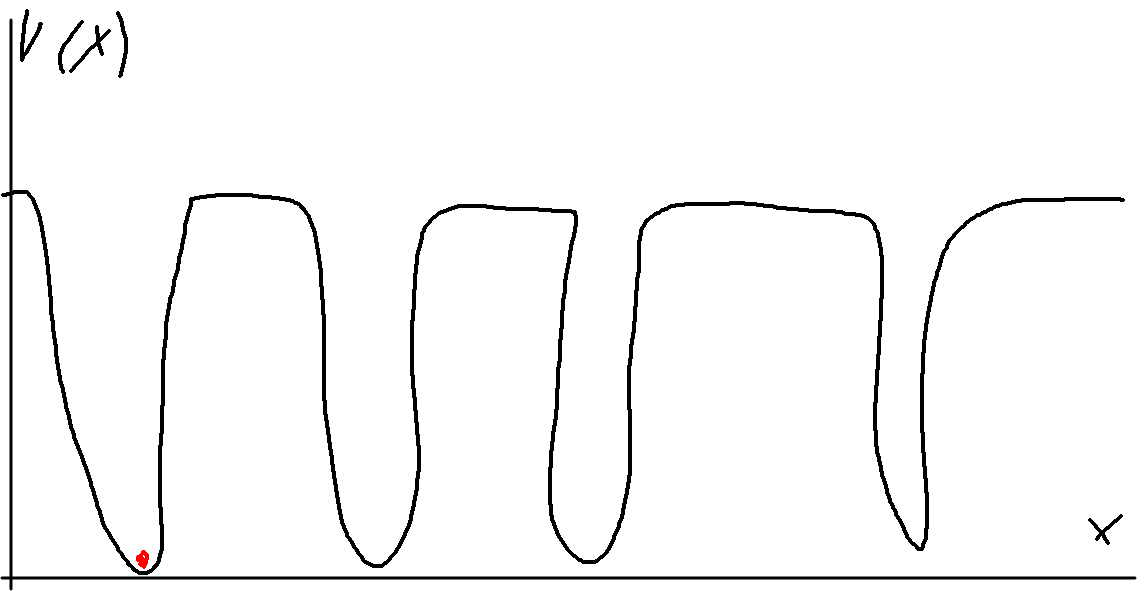
\includegraphics[width=\linewidth]{./lect4/pic1.png}
\end{center}
Particle can't get out of potential well though there are other well is could possible be into.

\paragraph{Meaning of ergodic hypothesis}
Suppose we have two closed Ising systems (with magnetic moments) and we connect them: one with $N_1=5$ and $2S_1=1$ and second with $N=10$ and $2S_2 = -2$.

Now, suppose we connected two systems to a single one.

If in each side nothing changes,
$$g^0_f = g_i = \frac{5!}{3!\cdot 2!} \cdot \frac{10!}{6!4!}$$

If one particle changes moment such that $2S_2 = 0$:
$$g^1_f = \frac{5!}{2!\cdot 3!} \cdot \frac{10!}{5!5!}$$
Note that $\frac{g_1^f}{g^0_f } = \frac{6}{5} > 1$.

If two particle changes moment such that $2S_2 = -2$:
$$g^2_f = \frac{5!}{1!\cdot 4!} \cdot \frac{10!}{6!3!}$$
Note that $\frac{g_1^f}{g^2_f } = \frac{6\cdot  \cdot 4}{ 5 \cdot 2 } > 1$.

Thus $g^1_f$ is most degenerated state, and the system will most of the time be on the most degenerated state. In big system, since variance of $X$ is $\frac{1}{\sqrt{N}}$, this state will observed almost always. I.e., there is flow from second box to the first one.

\paragraph{Example}
Now lets use Gaussian approximation. Then new degeneracy is
$g(N_1, S_1) \cdot g(N_2, S_2)$
and the condition is $S_1+S_2+S$. We also denote $N_1+N_2=N$. We are searching for a maximum of degeneracy under constrain.
$$g(N_1,N_2,S_1,S_2) = g_1(0)g_2(0) e^{-\frac{2S_1^2}{N_1}-\frac{2S_2^2}{N_2}}$$
Where $g_1(0)$, $g_2(0)$ are normalization constants, which doesn't affect optimization. Since $S_2 = S-S_1$:
$$g(N_1,N_2,S_1,S_2) = g_1(0)g_2(0) e^{-\frac{2S_1^2}{N_1}-\frac{2(S-S_1)^2}{N_2}}$$
We can optimize $\ln g$ instead, since, it's monotonous:
$$\ln g = C -\frac{2S_1^2}{N_1}-\frac{2(S-S_1)^2}{N_2} $$
$$\dv{\ln g}{S} =  -\frac{4S_1}{N_1}+\frac{4(S-S_1)}{N_2} = 0$$
$$N_1(S-S_1) - N_2 S_1= 0$$
$$N_1S - N S_1= 0$$
$$  S_1= \frac{N_1S}{N}$$
Thus
$$  S_2=  \frac{N_2S}{N}$$
How many states are in maximal degeneracy?

$$g(N_1,N_2,S_1,S_2) = g_1(0)g_2(0) e^{-\frac{2S^2}{N}}$$

Suppose we are looking at different state
$$\begin{cases}
S_1 = S_1^{max} + \delta
S_2 = S_2^{max} - \delta
\end{cases}$$
Then
$$g(N_1,N_2,S_1,S_2) = g_{max}(N_1,N_2,S_1,S_2) \cdot \exp\qty(-\frac{4S_1^{max} \delta}{N_1}-\frac{2\delta^2}{N_1}+\frac{4S_2^{max} \delta}{N_2}-\frac{2\delta^2}{N_2}) = g_{max}(N_1,N_2,S_1,S_2) \cdot \exp\qty(-\frac{2\delta^2}{N_1}-\frac{2\delta^2}{N_2})$$
For example, if $N_1=N_2=10^{22}$  and $\delta = 10^{12}$, i.e., $\frac{\delta}{N_1} = 10^{-10}$, 

$$g(N_1,N_2,S_1,S_2) = g_{max}(N_1,N_2,S_1,S_2) \cdot e^{-400}$$
\paragraph{General case}
Given two systems with degeneracy $g_1(N_1, U_1)$ and $g_2(N_2, U_2)$. $U_1+U_2 = U = \text{const}$ and $N_1=\text{const}$, $N_2=\text{const}$. We want to find maximal degeneracy:
$$\dv{U_1} g_1\cdot g_2 = \pdv{g_1}{U_1 } \cdot g_2 + \pdv{g_2}{U_2} \cdot \underbrace{\pdv{U_2}{U_1}}_{-1} \cdot g_1 = 0$$
$$\pdv{g_1}{U_1 }  \cdot \frac{1}{g_1} = \pdv{g_2}{U_2}  \cdot \frac{1}{g_2}$$
$$\pdv{\ln g_1}{U_1 }  = \pdv{\ln g_2}{U_2} $$
\paragraph{Temperature}
$$\frac{1}{T} = k_B + \pdv{U} \ln g$$
Define entropy (up to constant factor $k_B$)
$$\sigma = \ln g(N,U)$$
We also define
$$\frac{1}{\tau} = \frac{1}{k_B T} = \pdv{\sigma}{U}$$
If the system is continuous, we define number of states in some small interval as $\delta E$, then entropy is
$$\sigma = \ln \qty(g(N,U)\delta E)$$
and
$$\frac{1}{k_B T} = \pdv{\sigma}{U} = \pdv{U} \ln g + \underbrace{\pdv{U} \ln \delta E}_{\delta E = \text{const} \Rightarrow 0}$$
Also, define heat
$$\dd{Q} = \tau \dd{\sigma}$$
% \section{Thermodynamics}
\paragraph{Assumptions of thermodynamics}
\begin{enumerate}
	\item Heat is form of energy
	\item With high probability, the entropy of (non-equilibrium) closed system grows with time.
	\item When $\tau \to 0$, $\sigma\to0$ (there is one state).
\end{enumerate}
\subsection{Boltzmann distribution}
Suppose we divide a closed system into two parts: system and reservoir: 
\begin{center}
	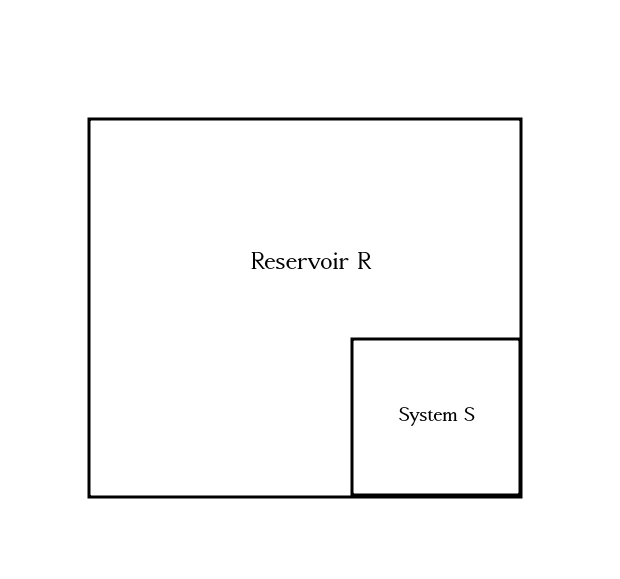
\includegraphics[width=0.5\linewidth]{./lect5/pic1.png}
\end{center}
What is probability that system $S$ will be in state which has energy $\epsilon$?
$$P_S(\epsilon)  \propto g_R(N,U_0 + \epsilon)$$
Where $U_0$ is total energy of reservoir + system. 
More precisely
$$P_S(\epsilon) = \frac{g_R(N,U_0 + \epsilon)}{g(U_0)}$$
For two states, ratio of probabilities is
$$\frac{P_S(\epsilon_1)}{P_S(\epsilon_2)} = \frac{g_R(N,U_0 - \epsilon_1)}{g_R(N,U_0 - \epsilon_2)} = e^{\sigma_R(U_0-\epsilon_1)-\sigma_R(U_0-\epsilon_2)}$$ 
We assume that reservoir is much larger than system, i.e., $U_0 \gg \epsilon_0$:
$$\sigma_R(U_0 -\epsilon) = \sigma_R(U_0) - \pdv{\sigma_R}{U}\epsilon + \order{\epsilon^2} \approx  \sigma_R(U_0) - \frac{1}{\tau} \epsilon$$
Thus

$$\frac{P_S(\epsilon_1)}{P_S(\epsilon_2)} = \frac{g_R(N,U_0 \cdot \epsilon_1)}{g_R(N,U_0 \cdot \epsilon_2)} = e^{-\frac{1}{\tau} (\epsilon_1-\epsilon_2)} = \frac{ e^{-\frac{\epsilon_1}{\tau}}}{ e^{-\frac{\epsilon_2}{\tau}}}$$ 
If we want for any $\epsilon$
$$P_S(\epsilon) \propto e^{-\frac{\epsilon}{\tau}}$$

We want to define the partition function:
$$Z(\tau) = \sum_{\text{states}} e^{-\frac{\epsilon_{\text{state}}}{\tau}}$$
and thus we normalize
$$P_S(\epsilon) = \frac{e^{-\frac{\epsilon}{\tau}}}{Z(\tau)}$$
this is called Boltzmann factor.

Such system is called canonical ensemble.
\subsection{Pressure}
Suppose we have microcanonincal ensemble of volume $V$ and dimensions $x$,$y$,$z$. If we move one of box walls by $\Delta z$, then we have
$$\underbrace{Pxy}_{F} \cdot (-\Delta z )= -P \Delta V  =\Delta W = \Delta E$$
We want energy difference to depend on two independent things - volume change and heat:
$$E = -P\Delta V + \tau \Delta \sigma$$
Thus we define
$$ P = - \eval{\pdv{E}{V}}_{N, \sigma}$$ 
We can rewrite
$$\dd{U} = \tau\dd{\sigma} - P\dd{V}$$
\paragraph{Ideal gas in 3D}
$$g(U,V,N) = \frac{3N}{2} V^N (2mU)^{\frac{3N}{2}-1} \frac{\pi^{\frac{3N}{2}}}{h^{3N} \Gamma\qty(\frac{3N}{2}+1)} $$
$$\sigma = \ln g = \ln \frac{3N}{2} + N\ln V + \qty(\frac{3N}{2}-1)\ln (2mU) - \ln \Gamma\qty(\frac{3N}{2}+1) - \ln \frac{\pi^{\frac{3N}{2}}}{h^{3N}}$$
Differentiating in implicit way
$$\dd{\sigma} = N \frac{1}{V} \ln \dd{V} +  \qty(\frac{3N}{2}-1)\frac{\dd{U}}{U} \approx N\frac{\dd{V}}{V} + \frac{3N}{2}\frac{\dd{U}}{U}$$
Since $\sigma$ is unchanged,
$$P = \pdv{U}{V} = -\frac{2}{3}\frac{U}{V}$$


Alternatively,
$$0 =\dd{\sigma} = \pdv{\sigma}{U}\dd{U} + \pdv{\sigma}{V} \dd{V}$$
$$\pdv{\sigma}{U} \pdv{U}{V} + \pdv{\sigma}{V} = 0$$
$$\frac{1}{\tau} (-P) + \pdv{\sigma}{V} = 0$$
$$\frac{P}{\tau} - \frac{N}{V} = 0$$
$$PV = k_B TN$$

\paragraph{}
Define $h = \frac{N}{N_A}$, for $N_A$ - Avogadro number, and also $R  = k_B N_A$, acquiring
$$PV = RhT$$
\section{Thermodynamical identities}
There are two kinds of variables: 
\begin{itemize}
	\item $\sigma$, $U$, $V$, $N$ - extensive variables. If we divide system, they change proportionally.
	
	Entropy representation:
	$$\begin{cases}
	\pdv{\sigma}{U} = \frac{1}{\tau}\\
	\pdv{\sigma}{V} = \frac{P}{V}
	\end{cases}$$
	\item $T$, $P$ are intensive variables. If we divide system, they don't change.
	$$\begin{cases}
	\pdv{U}{\sigma} = \tau\\
	\pdv{U}{V} = V
	\end{cases}$$
\end{itemize}

Define chemical potential $\mu=\pdv{U}{N}$ such that
$$\dd{U} = \tau \dd{\sigma} - P \dd{V} + \mu\dd{N}$$


$$\sigma(\lambda U, \lambda V, \lambda N) = \lambda \sigma ( U,  V,  N) $$
$$U(\lambda \sigma, \lambda V, \lambda N) = \lambda U (\sigma,  V,  N) $$
$$\qty(\pdv{U}{\lambda \sigma})_{V, N} \sigma + \qty(\pdv{U}{\lambda V})_{\sigma, N} V + \qty(\pdv{U}{\lambda N})_{\sigma, V} N  =U$$
Substituting $\lambda=1$ we get Euler equation:
$$U = \tau \sigma - PV + \mu N $$
Differentiating
$$\dd{U} = \sigma \dd{\tau} + \tau \dd{\sigma} -P\dd{V} -V\dd{P} + \mu \dd{N} + N\dd{\mu}$$
Remember the energy conservation
$$\dd{U} = \tau \dd{\sigma} - P \dd{V} + \mu\dd{N}$$
We get
$$0 = \sigma \dd{\tau} - V\dd{P} + N \dd{\mu}$$
This is called Gibbs–Duhem equation.

Note that we can't just add constant to energy, since it will not fulfill $U'(\lambda\sigma, \lambda V, \lambda N) = \lambda U'(\sigma, V, N)$. However, we can add a constant energy per particle.

\paragraph{Example}
Suppose we have microcanonical ensemble. The energy conserved $\dd{U} = 0$, and in optimal state entropy is maximal, thus $\dd{\sigma}=0$. Suppose we have some parameter $\pdv[2]{\sigma}{x} < 0$, for example moving wall of box.

Note that we can use entropy representation: start from maximal entropy $\dd{\sigma}=0$ and search for minimal energy $\dd{U}=0R$.

In entropy representation we get
$$\begin{cases}
\qty(\pdv{\sigma}{x})_U = 0\\
\qty(\pdv[2]{\sigma}{x})_U < 0\\
\end{cases}$$
In energy representation:
$$\qty(\pdv{U}{x})_\sigma = \frac{\qty(\pdv{\sigma}{x})_U}{\qty(\pdv{\sigma}{U})_x} = -\tau (\pdv{\sigma}{x})_U$$
Exists point $x_0$ such that $(\pdv{\sigma}{x})_U=0$. Since $\qty(\pdv{U}{x})_\sigma$ is increasing function, thus $\pdv[2]{U}{x}>0$, i.e. the point is minimum.

\paragraph{Canonical ensemble}
In canonical ensemble, we get
$$\begin{cases}
\dd{(U+U^r)} = 0\\
\dd{(\sigma+\sigma^r)} = 0\\
\end{cases}$$
If the system divided in two, we know that the reservoir can pass only heat to the system, thus:
$$\tau^r \dd{\sigma^r}+\tau^1 \dd{\sigma^1}+\tau^2 \dd{\sigma^1}=0$$
Since the whole microcanonical system (system+reservoir) is isolated:
$$\dd{\sigma^r}+\dd{\sigma^1}+ \dd{\sigma^2}=0$$
Subtracting:
$$(\tau^1-\tau^r) \dd{\sigma^1}+(\tau^2-\tau^r) \dd{\sigma^2}=0$$
This equality is always right, thus $\tau^1=\tau^2=\tau^r$.
Substituting $\dd{U^r}$:
$$\dd{U} + \tau^{r} \dd{\sigma^r} = 0$$
Substituting $\dd{\sigma^r} = -\dd{\sigma}$ and $\tau=\tau^r$:
$$\dd{U} - \tau \dd{\sigma} = 0$$ 
$$\dd{(U -\tau\sigma)}  = 0$$ 
Define new quantity, free energy:
$$F = U - \tau \sigma = U - TS$$

Note, that if we compress gas, its temperature increases, and this energy goes to the atmosphere (reservoir), and thus part of energy is lost. $F$ is extensive quantity.

Since $U^r$ depends only on $\tau$ and $\sigma$ we can rewrite

$$F = U(\tau, V, N) - \tau \sigma(\tau, V, N) $$
such that $F$ doesn't depend on properties of reservoir except temperature.
\paragraph{Constant pressure}
we can replace reservoir with ballon of gas such that the pressure will be kept constant. In this case we minimize a quantity called enthalpy:
$$H = U+PV$$
\subsection{Average energy in canonical case}
$$\expval{\epsilon} = \frac{\sum_{states} \epsilon_{st} e^{-\frac{\epsilon_{st}}{\tau}}}{Z(\tau)} = \tau^2 \pdv{\ln Z}{\tau}$$
Why is it true?
$$\pdv{\ln Z}{\tau} = \frac{1}{Z} \pdv{Z}{\tau} $$
Define $\beta = \frac{1}{\tau}$, then
$$\pdv{\tau} = -\frac{1}{\tau^2} \pdv{\beta}$$
$$\pdv{Z}{\tau} = -\frac{1}{\tau^2} \pdv{\beta} \sum e^{-\beta \epsilon_{st}} = \frac{1}{\tau^2} \sum_{states} \epsilon_{st} e^{-\beta \epsilon_{st}} $$
Thus
$$\pdv{\ln Z}{\tau} = \frac{1}{Z\tau^2} \sum_{states} \epsilon_{st} e^{-\frac{\epsilon_{st}}{\tau} }  $$
i.e.,
$$\expval{\epsilon} = \tau^2 \pdv{\ln Z}{\tau}$$
\paragraph{Magnetic moments with reservoir}
Suppose we have magnetic field $B$, denote
$$\mu B = \frac{1}{2} \epsilon$$
If we have exactly two moments,
$$Z_1 = e^{-\frac{\epsilon}{2\tau}}+e^{\frac{\epsilon}{2\tau}} = 2\cosh(\frac{\epsilon}{2\tau})$$
and
$$Z_2 = \qty( e^{-\frac{\epsilon}{2\tau}}+e^{\frac{\epsilon}{2\tau}} )\qty( e^{-\frac{\epsilon}{2\tau}}+e^{\frac{\epsilon}{2\tau}} ) $$
And in general,
$$Z_N = Z_1^N$$

For one particle:
$$\expval{\epsilon_1} = \frac{-\frac{1}{2} \epsilon e^{\frac{\epsilon}{2\tau}}+\frac{1}{2} \epsilon e^{-\frac{\epsilon}{2\tau}}}{ e^{-\frac{\epsilon}{2\tau}}+e^{\frac{\epsilon}{2\tau}}} = -\frac{\epsilon}{2} \frac{\sinh(\frac{\epsilon}{2\tau})}{\cosh(\frac{\epsilon}{2\tau})} = -\frac{\epsilon}{2}\tanh(\frac{\epsilon}{2\tau})$$

Now for $N$ particles
$$\expval{\epsilon} = \tau^2 \pdv{\ln Z}{\tau} \tau^2 \pdv{\tau} \ln Z_1^N = N \cdot \tau^2 (\frac{\epsilon}{2\tau}) = N \expval{\epsilon_1}$$
\paragraph{Thermodynamic perspective}
Define $2S = N^{\uparrow} - N^{\downarrow}$.
$$g(N,S) = \frac{N!}{N^{\uparrow}! N^{\downarrow}!}$$
$$\sigma(N,S) = \ln g(N,S) = \frac{1}{2} \ln(2\pi N)^{-1} - \qty(\frac{1}{2}N+S) \ln(\frac{1}{2}+\frac{S}{N}) -\qty(\frac{1}{2}N-S ) \ln(\frac{1}{2} + \frac{S}{N})$$
Thus
$$F = U -\tau \sigma = -2\mu BS - \frac{\tau}{2} \ln(2\pi N)^{-1}+ \qty(\frac{1}{2}N+S)\tau \ln(\frac{1}{2}+\frac{S}{N}) +\qty(\frac{1}{2}N-S )\tau \ln(\frac{1}{2} + \frac{S}{N}) $$ 
$$\pdv{F}{S} = -2\mu B +\tau \ln(\frac{N+2S}{N-2S}) = 0$$
$$\frac{N+2S}{N-2S} = e^{\frac{2\mu B}{\tau}}$$
$$N+2S = (N-2S)e^{\frac{2\mu B}{\tau}}$$
$$2S\qty(1+e^{\frac{2\mu B}{\tau}}) = N\qty(e^{\frac{2\mu B}{\tau}}-1)$$
$$2S = N\frac{e^{\frac{2\mu B}{\tau}}-1}{1+e^{\frac{2\mu B}{\tau}}}$$
$$2S = N\frac{e^{\frac{\mu B}{\tau}}-e^{-\frac{\mu B}{\tau}}}{e^{-\frac{\mu B}{\tau}}+e^{\frac{\mu B}{\tau}}} = N\frac{\sinh(-\frac{\mu B}{\tau})}{\cosh(-\frac{\mu B}{\tau})} =N \tanh(-\frac{\mu B}{\tau})$$
Since $\epsilon = -2\mu B S$
$$\epsilon = -\mu B N  \tanh(-\frac{\mu B}{\tau})$$
\paragraph{Connection between $F$ and $Z$}
$$F = U -\tau \sigma$$
$$\dd{F} = \dd{U} -\sigma \dd{\tau} - \tau \dd{\sigma}$$
$$\dd{U} = \tau \dd{\sigma} - P\dd{V}$$
i.e.,
$$\dd{F} = -P\dd{V} - \sigma\dd{\tau}$$
Thus, if $\tau$ is constant
$$\dd{F} =- P\dd{V}$$
$$P = -\qty(\pdv{F}{V})_{\tau}$$
If, on contrary, volume is constant
$$\sigma = -\qty(\pdv{F}{\tau})_{V}$$
If we differentiate first equation, with constant $\tau$, we get
$$\qty(\pdv{F}{V})_{\tau} +\qty(\pdv{U}{V})_{\tau} = \tau\qty(\pdv{\sigma}{V})_{\tau} \Rightarrow -P = \qty(\pdv{U}{V})_{\tau} -\tau\qty(\pdv{\sigma}{V})_{\tau}$$
i.e.,
$$P = -\qty(\pdv{U}{V})_{\tau} +\tau\qty(\pdv{\sigma}{V})_{\tau}$$

In addition, substituting $\sigma$:

$$F = U  + \tau\qty(\pdv{F}{\tau})_{V} $$
$$U = F - \tau\qty(\pdv{F}{\tau})_{V}$$
$$U =- \tau^2 \qty[ \pdv{\tau} \frac{F}{\tau}]$$
At the same time
$$U = -\tau^2 \pdv{\ln Z}{\tau}$$
$$- \tau^2 \qty[ \pdv{\tau} \frac{F}{\tau}]  = -\tau^2 \pdv{\ln Z}{\tau}$$
$$ \frac{F}{\tau}  = -\ln Z + \alpha(V)$$
for some constant $\alpha$ depending on volume, and thus we conclude that $\expval{\epsilon} = U$.
\paragraph{Quantum particle in box}
Suppose we have particle in box, it has energy
$$E=\frac{\hbar^2}{2m} \qty(\frac{\pi}{2})^2 n^2$$
Note here we have minimal energy which is non-zero, and for this energy we have only one possible state, which confirms third law of thermodynamics (in opposite, in classical mechanics there are many states with minimal energy).

In limit $Z\to 0$ we get
$$Z = g_0e^{\frac{\epsilon_0}{Z}} +\sum_{\text{high energies}} e^{-\frac{\epsilon}{Z}} \approx  g_0e^{\frac{\epsilon_0}{Z}}$$
From third law $g_0=1$.
$$\ln Z = -\frac{\epsilon_0}{Z}$$
$$F = -\tau \ln Z + \alpha \tau = \epsilon_0 +\alpha \tau$$
Since 
$$\sigma = -\qty(\pdv{F}{\tau})_V$$
$$\sigma=-\alpha$$
i.e., $\alpha = 0$, meaning
$$F= -\tau \ln Z$$
\subsection{Classical ideal gas in statistic approach}
In thermodynamics we acquired 
$$PV=Nk_BT$$
$$U=\frac{3}{2} Nk_BT$$
$$g(U,V) =V^N U^{\frac{3}{2}N-1}$$
\paragraph{Partittion function of ideal gas}
\begin{align*}
	Z_N = \frac{1}{h^{3N}} \int \dd{p_x^1} \int \dd{p_y^1} \int \dd{p_z^1} \dots  \int \dd{p_x^N} \int \dd{p_y^N} \int \dd{p_z^N} \int \dd{x_1} \int \dd{y_1} \int \dd{z_1} \dots  \int \dd{x_N} \int \dd{y_N} \int \dd{z_N} e^{-\frac{1}{z} \sum_{i=1}^N \frac{\va{p}_i^2}{2m\tau}} =\\=
	\frac{V^n}{h^{3N}} \int \dd{p_x^1} \int \dd{p_y^1} \int \dd{p_z^1} \dots  \int \dd{p_x^N} \int \dd{p_y^N} \int \dd{p_z^N} e^{-\frac{1}{z} \sum_{i=1}^N \frac{\va{p}_i^2}{2m\tau}} =\\=
	\frac{V^n}{h^{3N}} \int \dd{p_x^1} \int \dd{p_x^1} e^{-\frac{1}{z} \frac{{p_x^1}^2}{2m\tau}} \int \dd{p_y^1} e^{-\frac{1}{z} \frac{{p_y^1}^2}{2m\tau}} \int \dd{p_z^1} e^{-\frac{1}{z} \frac{{p_z^1}^2}{2m\tau}} \dots  \int \dd{p_x^N} e^{-\frac{1}{z} \frac{{p_x^N}^2}{2m\tau}} \int \dd{p_y^N} e^{-\frac{1}{z} \frac{{p_y^N}^2}{2m\tau}} \int \dd{p_z^N} e^{-\frac{1}{z} \frac{{p_z^N}^2}{2m\tau}}
\end{align*}

Then for each particle
$$Z_1 = \frac{V}{h^{3}} \int \dd{p_x^1}  \int \dd{p_x^1} e^{-\frac{1}{z} \frac{{p_x^1}^2}{2m\tau}} \int \dd{p_y^1} e^{-\frac{1}{z} \frac{{p_y^1}^2}{2m\tau}} \int \dd{p_z^1} e^{-\frac{1}{z} \frac{{p_z^1}^2}{2m\tau}} = \frac{V}{h^{3}} \qty[\int_{-\infty}^\infty \dd{p} e^{- \frac{p^2}{2mz\tau}}]^3 \stackrel{\text{Gaussian}}{=}  \frac{V\qty(2\pi m \tau )^{\frac{3}{2}}}{h^{3}}$$
$$Z_N = Z_1^N$$
$$\expval{\epsilon} = \tau^2 \pdv{\ln Z_n}{\tau} = \tau^2 N \pdv{\ln Z_1}{\tau} = \tau^2 N \cdot \frac{3}{2\tau} = \frac{3}{2} N\tau = \frac{3}{2} Nk_BT$$
\paragraph{Pressure of ideal gas}
$$P = -\qty(\pdv{F}{V})_\tau $$
And
$$F = -\tau \ln Z_N = -\tau \ln Z_1^N = -\tau N \ln Z_1 = -\tau N \qty(\ln(V) + \ln (\tau^{\frac{3}{2}}) + \text{const})$$
$$\pdv{F}{V} = -\frac{\tau N}{V}$$
$$P = \frac{\tau N}{V}$$
$$PV = \tau N = k_B NT$$
\subsection{Second law. Maxwell demon}
\paragraph{Second law} 
\begin{enumerate}
	\item Heat transfers from warm to cold
	\item Carnot engine has maximal efficiency 
	\item Entropy of closed system can only increase, i.e. $\dot{S}\geq0$. To proof it, we need that movement laws are symmetric in time.
	\item It's impossible to get work from a single temperature source.
\end{enumerate}
\paragraph{Forbidding laws of physics }
\begin{enumerate}
	\item Energy conservation. For
	 $$E = \sum_i \frac{p_i^2}{2m_i}+ \sum_i V(\va{r}_i) + \sum_{i\neq j} V_{ij}$$
	 This law prohibits existence of perpetuum mobile. It's equivalent to first law of thermodynamics.
\end{enumerate}


\begin{center}	
	\includesvg[eps,svgpath = lect10/,width=0.5\linewidth]{pic1}
\end{center}
Each of $T_C$, $T_H$, performs work equals to change in heat $\Delta VP = \Delta Q$. Then total work is 
$$W_{total} = \Delta Q_c - \Delta Q_h$$
Carnot showed that
$$\frac{W}{\Delta Q_h} \leq 1 - \frac{T_c}{T_h}$$

\paragraph{Maxwell demon}
Since $\frac{3}{2}Nk_BT = \frac{1}{2} \sum_i m\va{v}_i^2$.

\begin{center}	
	\includesvg[eps,svgpath = lect10/,width=0.5\linewidth]{pic2}
\end{center}

Suppose we have a demon that can allow only fast particles from right to left and only slow particles from left to right. 

Alternatively, he can only allow particles from left to right, and thus change the pressure in two parts.
\subsection{Equipartition theorem}
Let $f$ number of degrees of freedom and $o_i$ - $i^{th}$ degree of freedom, then
$$E = \sum_{i=1}^f a_io_i^2$$

\paragraph{Example: harmonic oscillator}
First $\frac{f}{2}$ degrees of freedom are momenta and second half are locations
$$Z = \frac{1}{h^f}  \idotsint_{-\infty}^\infty \dd{o_1} \dots \dd{o_{\frac{f}{2}}} \dd{o_{\frac{f}{2}+1}}\dots \dd{o_f} e^{-\beta \sum_{i=1}^f a_io_i^2} = \prod_{i=1}^f \frac{1}{h} \int_{-\infty}^\infty e^{-\beta a_io^2} \dd{o}  = \prod_{i=1}^f \frac{1}{h} \sqrt{\frac{\pi \tau}{a_i}}$$
$$\expval{\epsilon} =c\tau^2 \pdv{\tau} \ln Z = \tau^2 \pdv{\tau} \sum_{i=1}^f \ln(\frac{1}{h} \sqrt{\frac{\pi \tau}{a_i}}) = \tau^2 \pdv{\tau} f\ln \tau^{\frac{1}{2}} = \frac{1}{2} \tau f$$

Note that we count only degrees of freedom which can acquire values from $-\infty$ to $\infty$, thus, for ideal gas $f=3N$ (for oscillators $f=6N$).
\paragraph{Definition} Interaction is part of energy that depends on distance between particles:
$$E = \sum \frac{p_i^2}{2m} + V(r_i) + \sum_j U(\va{r}_i-\va{r}_j)$$
\subsection{Thermodynamic potentials}
\paragraph{Electric potential}
Electric potential is $\phi(x,y)$ such that
$$\dd{\phi} = \pdv{\phi}{x} \dd{x} \pdv{\phi}{y} \dd{y}$$
Electric field is $E = -\grad{\phi}$ and its conserving field, i.e. $\curl{\va{E}} = 0$.
\paragraph{In thermodynamics}
$F$, $\sigma$, $u$ are potential in sense that difference between two states is independent on path.

\paragraph{1D}
$$\dd{F} = \qty(\pdv{F}{\tau})_V \dd{\tau} + \qty(\pdv{F}{V})_\tau \dd{V}$$
$$\dd{U} = \underbrace{\qty(\pdv{U}{\sigma})_V}_{\tau} \dd{\sigma} + \underbrace{\qty(\pdv{F}{V})_\sigma}_{-P} \dd{V}$$
If $U$ is potential then
$$\qty[\pdv{V} \qty(\pdv{U}{\sigma})_V]_\sigma =\qty[ \pdv{\sigma} \qty(\pdv{U}{V})_\sigma]_V$$
$$\qty(\pdv{T}{V})_\sigma = -\qty(\pdv{P}{\sigma})_V$$

Additional example:
$$\qty[\pdv{V} \qty(\pdv{U}{\sigma})_V]_\sigma =\qty[ \pdv{\sigma} \qty(\pdv{U}{V})_\sigma]_V$$
$$\qty(\pdv{T}{V})_\sigma = -\qty(\pdv{P}{\sigma})_V$$

Also, similarly to electricity, the path integral is potential difference:
$$\Delta F = \int_{V_0,\tau_0}^{V_1, \tau_1} -\sigma \dd{\tau} - P \dd{V}$$
\paragraph{Gibbs free energy}
Experimental system is in constant temperature and pressure. Instead of searching for total entropy, we'll try something else:
$$U^\dagger = U^r+U^1+U^2$$
$$\begin{cases}
\dd{U}^\dagger = \dd{U}^r + \dd{U}^1 + \dd{U}^2\\
\dd{\sigma}^r+ \dd{\sigma}^1 + \dd{\sigma}^2 = 0\\
\dd{V}^1+\dd{V}^2+\dd{V}^r = 0\\
\dd{V}^1+\dd{V}^2 = 0
\end{cases}$$
Substituting energy:
$$\tau^r\dd{\sigma}^r + \tau^1\dd{\sigma}^1 + \tau^2\dd{\sigma}^2 - P^r\dd{V}^r  - P^1\dd{V}^1  - P^2\dd{V}^2 + \mu^1 \dd{N}^1 + \mu^2 \dd{N}^2 = 0$$
$$(\tau^1-\tau^r)\dd{\sigma}^1 + (\tau^2-\tau^r)\dd{\sigma}^2 + (P^r-P^1) \dd{V}^1 + (P^r-P^2) \dd{V}^2 + (\mu^1-\mu^2)\dd{N}^1 = 0$$
$$\begin{cases}
\tau^2=\tau^r=\tau^1\\P^1=P^2=P^r\\\mu^1=\mu^2
\end{cases}$$
Thus we'll optimize
$$G=U-\tau\sigma+PV$$

 For isolated system,
$$U = \tau \sigma - PV + \mu N$$
$$G = \mu N$$

\paragraph{Second derivatives of $G$}
$$G(\tau, P, N) = U(\tau, P, N) - \tau \sigma(\tau, P, N) -  PV(\tau, P, N)$$
In ideal gas, temperature defines energy:
$$\dd{G} =\dd{U} - \tau \dd{\sigma} - \sigma \dd{\tau} + P\dd{V} +V\dd{P}$$
From energy conservation
$$\dd{U} =  - \sigma \dd{\tau} + P\dd{V} +\mu\dd{N}$$
$$\dd{G} = - \sigma \dd{\tau} + V\dd{P} + \mu \dd{N}$$
$$\qty(\pdv{G}{\tau})_{P,N} = -\sigma \quad \qty(\pdv{G}{P})_{\tau,N} = V \quad \qty(\pdv{G}{N})_{P,\tau} = \mu$$
Thus $G$ is potential:
$$\pdv{G}{\tau}{P} = \pdv{G}{p}{\tau} \Rightarrow \qty(\pdv{\tau} V)_P = -\qty(\pdv{P} \sigma)_\tau$$
\paragraph{Measurable quantities}
It's hard to measure energy or entropy, thus we'll measure different quantities:

\begin{itemize}
	\item Compressibility
	$$k_T(T,P) = -\frac{1}{V} \qty(\pdv{V}{P})_{T,N}$$
	Coefficient of thermal expansion:
	$$\alpha(\tau,P) = \frac{1}{V} \qty(\pdv{V}{T})_{P,N}$$
	Specific heat:
	$$c_P = \frac{1}{N} \qty(\frac{\delta Q}{\dd{T}})_{P,N}$$
\end{itemize}

Here, $\delta Q$ is inexact differential, meaning that $Q$ is path function (depends on path taken to get from one state to another), or alternatively, there doesn't exists a function $q$ such that $\grad{q}=Q$.
\paragraph{$\alpha, k_T, c_P$ are useful for non-ideal gas}
In ideal gas there are no interactions, thus everything we solved can't be applied for non-ideal gases.
\paragraph{$N$ atoms in volume $V$}
$$V = V(\tau,P)$$
$$\dd{V} = \qty(\pdv{V}{P})_\tau \dd{P} +\qty(\pdv{V}{\tau})_P \dd{\tau}$$
$$\dd{V}b= -Vk_{\tau}(\tau,P) \dd{P} + V\alpha(\tau, P) \dd{\tau}$$
$$\int_{V_0,\tau_0}^V \frac{\dd{V}}{V} = \int_{\tau_0,P_0}^{\tau, P} \begin{pmatrix}-k_{\tau}(\tau,P) \dd{P} & \frac{1}{k_B}\alpha(\tau, P)\end{pmatrix}\begin{pmatrix}
\dd{P}\\\dd{\tau}
\end{pmatrix}$$
$$\ln(\frac{V}{V_0}) = \int_{\tau_0}^\tau \frac{\alpha}{k_B} (\tau', P_0) \dd{\tau'} - \int_{P_0}^P k_T (T,P') \dd{P'}$$
\paragraph{Quantum gas}
One dimentional Shr\"{o}dinger equation
$$-\frac{\hbar^2}{2m} \pdv[2]{\Psi}{x} = E\Psi$$
$$\Psi = A\sin(kx)$$
when $kL = n\pi$.
$$E = \frac{\hbar^2 k^2}{2m} = \frac{\hbar^2}{2m} \qty(\frac{\pi}{L})^2n^2$$
In 3D we get
$$-\frac{\hbar^2}{2m} \laplacian{\Psi}{x} = E\Psi$$
$$\Psi = A\sin(k_xx)\sin(k_yy)\sin(k_zz)$$
Each of $k_i = \qty(\frac{\pi}{L})n_i$, i.e.
$$E = \frac{\hbar^2}{2m} \qty(\frac{\pi}{L})^2\qty(n_x^2+n_y^2+n_z^2)$$
\end{document}
